\import{./}{exempt-delegation-attack-diagram.tex}

\section{Exempt Delegations}

Exempt delegations (proposed in LSM~\cite{liquidity-staking-module})
are a mechanism to alleviate the Principal--Agent problem in liquid staking.
An exempt delegation amount $c$, measured in \asset, is associated
with each validator. It is a measure of the validator's trustworthiness.
The liquid staking protocol is now redesigned to impose restrictions
on how much of the protocol's pooled moneys can be delegated to a particular
validator based on the validator's exempt delegation.
The restriction is
parameterized by a factor $\phi$ (in practice, $\phi > 1$)
and is given by the inequality $b \leq \phi c$: Only up to $b$ \assets
are allowed to be delegated by the liquid staking protocol
to a validator with $c$ \assets in exempt delegations.

A new validator begins its lifecycle with $c = 0$. They can then
raise their own exempt delegation amount by locking aside a
chosen amount of \asset, and marking it as \emph{exempt}. Those
assets are delegated to the validator as usual. However,
the \emph{exempt}
marking means that those delegated assets cannot be part of the liquid
staking protocol pool, but must remain infungibly locked aside. Additionally,
these specially marked delegations are slashed\footnote{We abstract some
of the irrelevant implementation details here. See Section~\ref{sec:lsm}
for how the real protocol works in the context of Cosmos.}
at a potentially higher rate $q \geq p$. Exempt delegated assets cannot
be undelegated in a way that would cause a violation of the inequality
$b \leq \phi c$.

Delegators, whether wise or unwise, do not participate in exempt
delegations; instead, it is the validator who exempt delegates to
themselves (or someone who trusts the validator for extrinsic reasons).
This means that, in case of validator misbehavior, the exempt delegation
slashing $qc$ is a penalty that only affects the validator.

This raises
the cost of the attack described in the previous section. The
adversary must first, at time $t_1$ (where $t_0 < t_1 < t_2$), exempt delegate a sufficient amount
$c \geq \frac{b}{\phi}$ \asset to $\mathcal{V}$ before she can liquid stake $b$ \asset.
Whereas the \stassets
corresponding to those $b$ \assets can be, as before, sold at $t_3$ to
separate the Agent from the Principal, the $c$ amount remains with the
Agent, holding her financially liable to misbehavior. After equivocation at $t_4$,
in addition to any other costs, the adversary loses $qc$ \asset. At the conclusion
% Maybe before closing her position?
of the attack, the adversary undelegates the remaining $(1 - q)c$ exempt delegation.
The timeline of the attack is illustrated in Figure~\ref{fig:exempt-timeline}.

The attack may remain profitable despite exempt delegations.
The rational adversary should not waste any unnecessary resources on
$c$; therefore, she can set $c = \frac{b}{\phi}$. The profit of the attack now
becomes $b^* - b' - \frac{q}{\phi}b$.
The intuition for why exempt delegations protect the system is that,
for the adversary to profit from the short, she must cause a significant
shift in the price. The shift in the price is determined by the factor
$p\frac{b}{b_0}$, so the adversary aims for a large $b$. But because $b \leq \phi c$
must be respected, this incurs a large penalty $qc = \frac{q}{\phi}b$.

% TODO: Consider the adverasary taking a loan up to s_0 asset and using the rest of u
% just to move the market
\noindent
\textbf{Initial capital}
Let $\gammastasset$ be the collateral ratio of a standard \stasset
loan.
To perform the attack, the adversary has an initial capital of $u$ \asset.
She will use this as collateral to get the $z = \frac{u}{\gammastasset} \frac{s_0}{b_0}$ \stasset
loan, needed to short \stasset at $t_0$.
% Talk about collateral ratio in preliminaries
After converting the loaned $z$ \stasset to $b^*=\frac{u}{\gammastasset}$ \asset, part
of the funds are used to exempt delegate $c = \frac{b}{\phi}$ \asset
to $\mathcal{V}$. Another part
is used to obtain the required $b$ \asset using a flash loan. The cost of
the flash loan is $\betaasset b$. Hence:
% TODO: Maybe only a flash loan could be used instead of loan?

\begin{gather*}
  c + \betaasset b \leq b^*\Rightarrow\\
  \frac{b}{\phi} + \betaasset b \leq b^*\Rightarrow\\
  b \leq \frac{u}{(\frac{1}{\phi} + \betaasset)\gammastasset}
\end{gather*}

The final profit of the attack is $\alpha = b^* - b' - qc - \betaasset b$.
Solving for $\frac{d\alpha}{db} = 0$ gives the optimal $b = \sqrt{\frac{u f p b_0}{(\betaasset + \frac{q}{\phi})\gammastasset}} - b_0$,
which maximizes
the adversary's profit, subject to the constraints
$0 \leq b \leq \frac{u}{(\frac{1}{\phi} + \betaasset) \gammastasset}$.
In non-extreme market conditions, if the attack is profitable, the bound
$b \leq \frac{u}{(\frac{1}{\phi} + \betaasset)\gammastasset}$ will not be reached,
and the adversary will use the value
$b = \sqrt{\frac{u f p b_0}{(\betaasset + \frac{q}{\phi})\gammastasset}} - b_0$.


Solving $\alpha = 0$ for $\frac{q}{\phi}$ with $b\geq0$ gives the
security parameter of the protocol.

% (-b0*β*γ - 2*sqrt(f)*sqrt(p)*u*sqrt(f - 1) + f*p*u + f*u - u)/(b0*γ)
% (1/(b0*γ)) * (f*p*u + f*u - b0*β*γ - 2*u*sqrt(fp*(f-1)) - u)
\begin{gather*}
  \frac{\phi}{q} \leq \frac{b_0 \gammastasset}{f p u + f u - b_0 \betaasset \gammastasset - 2 u \sqrt{fp (f-1)} - u}
\end{gather*}

This parameter should be calculated independently for each protocol by replacing
the constants: $p$, $\betaasset$, $f$, $b_0$, $\gammastasset$ and $u$ with the
appropriate values of the blockchain it operates on.

Higher slashing of exempt delegations $q$ makes the protocol more secure. This
is because more of the exempt delegation $c$, holding the adversary accountable,
is slashed. Lower exempt delegation factor $\phi$ also makes the protocol more secure.
A larger exempt delegation $c$ is required to liquid stake $b$ \asset.
Hence, lower $\frac{\phi}{q}$ makes the protocol less vulnerable to the attack.


We consider: a blockchain with slashing percentage $p = 0.5$, an \asset market
with flash loan cost $\betaasset = 0.003$, a \stasset market with total
loan cost $f = 1.03$ for duration $\Delta_z$ and collateral ration
$\gammastasset = 1.2$. The initial \asset holdings of the liquid staking protocol
are $b_0 = 10000$ \asset.

While the cost of borrowing money goes up, the attack becomes less profitable
for the adverasary. Thus, the protocol has to increase the parameter
$\frac{\phi}{q}$ to remain secure.

\begin{figure}[htb]
  \centering
  \begin{subfigure}{0.49\textwidth}
    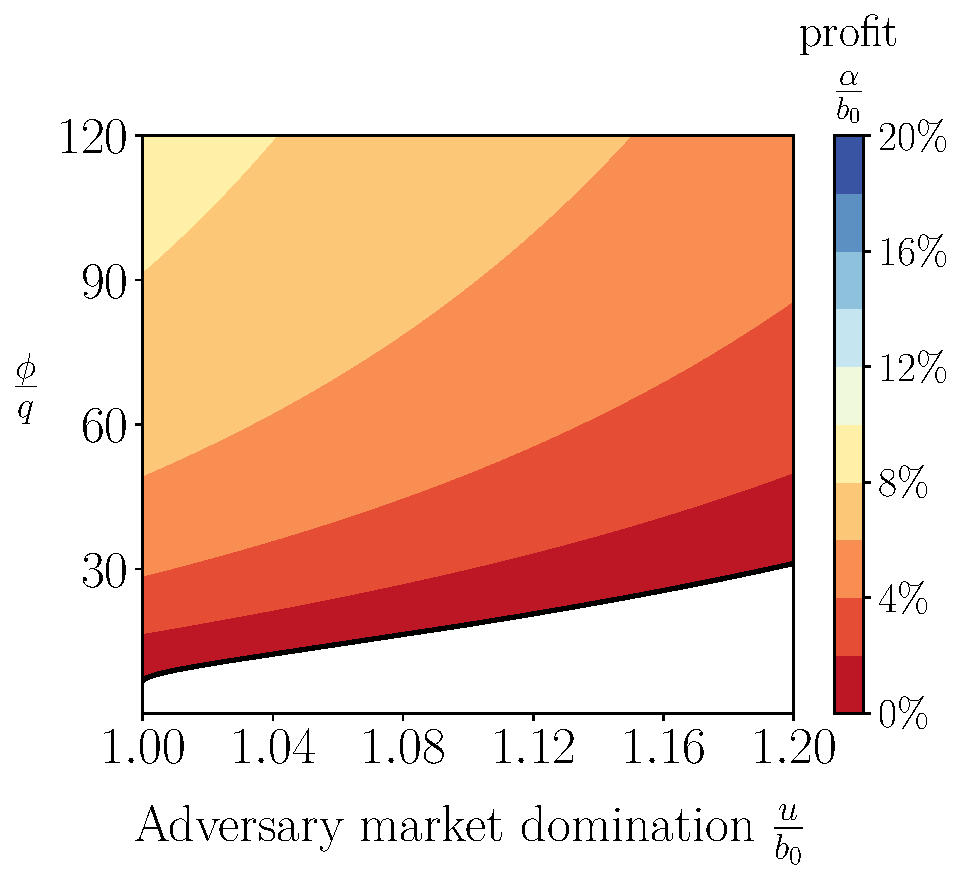
\includegraphics[width=\textwidth]{./plots/plotf30.pdf}
    \caption{Collateral $u = 30\%$ of $b_0$.}
    \label{fig:plotf30}
  \end{subfigure}
  \hfill
  \begin{subfigure}{0.49\textwidth}
    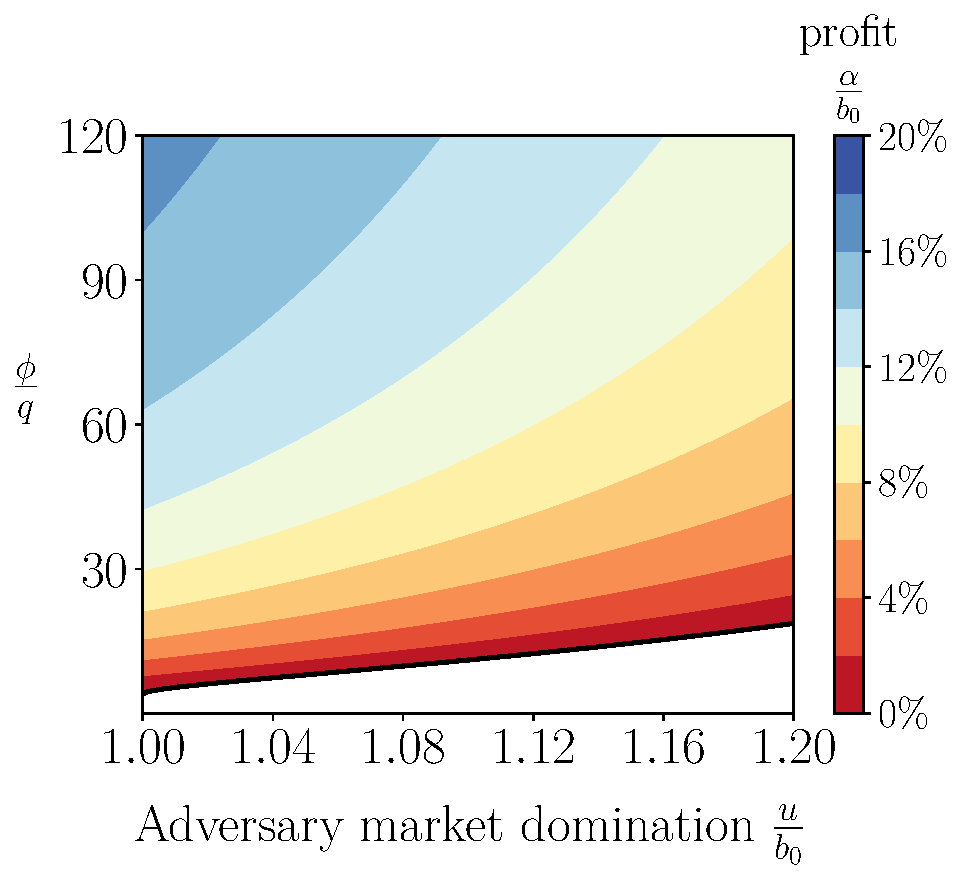
\includegraphics[width=\textwidth]{./plots/plotf50.pdf}
    \caption{Collateral $u = 50\%$ of $b_0$.}
    \label{fig:plotf50}
  \end{subfigure}
  \caption{Attack profitability.}
  \label{fig:images}
\end{figure}

%\begin{align*}
%  &a = b^* - b' - qc - \betaasset b\\
%  &a = \frac{b_0}{s_0}z(1 - (1 - p\frac{b}{b_0 + b})((1 + \rstasset)^{\Delta_z} + \betastasset)) - \betaasset b - \frac{q}{\phi}b\\
%  &a = \frac{u}{\gammastasset}(1 - (1 - p\frac{b}{b_0 + b})((1 + \rstasset)^{\Delta_z} + \betastasset)) - \betaasset b - \frac{q}{\phi}b\\
%\end{align*}
%
%Let $f = (1 + \rstasset)^{\Delta_z} + \betastasset$:
%
%\begin{align*}
%  &a = \frac{u}{\gammastasset}(1 - (1 - p\frac{b}{b_0 + b})f) - \betaasset b - \frac{q}{\phi}b\\
%\end{align*}

%\begin{gather*}
%  \frac{da}{db} = 0\\
%  \frac{u f p}{\gammastasset} \frac{b_0}{(b_0 + b)^2} - \betaasset - \frac{q}{\phi} = 0\\
%  \frac{u f p b_0}{\gammastasset (b_0 + b)^2} = \betaasset + \frac{q}{\phi}\\
%  \frac{u f p b_0}{\gammastasset (\betaasset + \frac{q}{\phi})} = (b_0 + b)^2\\
%  (b_0 + b)^2 - \frac{u f p b_0}{\gammastasset (\betaasset + \frac{q}{\phi})} = 0\\
%  b^2 + 2b_0b + b_0^2 - \frac{u f p b_0}{\gammastasset (\betaasset + \frac{q}{\phi})} = 0\\
%\end{gather*}

%The solution for $b > 0$ is:
%$b = \sqrt{\frac{u f p b_0}{\betaasset + \frac{q}{\phi}}} - b_0$


% TODO: analyze rationality of the attack
% TODO: appendix? introduce discount of stasset -> asset in the market using loans
